% Тут используется класс, установленный на сервере Papeeria. На случай, если
% текст понадобится редактировать где-то в другом месте, рядом лежит файл matmex-diploma-custom.cls
% который в момент своего создания был идентичен классу, установленному на сервере.
% Для того, чтобы им воспользоваться, замените matmex-diploma на matmex-diploma-custom
% Если вы работаете исключительно в Papeeria то мы настоятельно рекомендуем пользоваться
% классом matmex-diploma, поскольку он будет автоматически обновляться по мере внесения корректив
%

% По умолчанию используется шрифт 14 размера. Если нужен 12-й шрифт, уберите опцию [14pt]
% \documentclass[14pt]{matmex-diploma}
\documentclass[14pt]{matmex-diploma-custom}

\begin{document}
% Год, город, название университета и факультета предопределены,
% но можно и поменять.
% Если англоязычная титульная страница не нужна, то ее можно просто удалить.
\filltitle{ru}{
    chair              = {Программная инженерия},
    title              = {Интеграция программирования на языке Python в образовательные решения TRIK},
    % Здесь указывается тип работы. Возможные значения:
    %   coursework - Курсовая работа
    %   diploma - Диплом специалиста
    %   master - Диплом магистра
    %   bachelor - Диплом бакалавра
    type               = {bachelor},
    position           = {студента},
    group              = 471,
    author             = {Белков Роман Владимирович},
    supervisorPosition = {ст.\, преп.\,},
    supervisor         = {Я.\,А. Кириленко},
    reviewerPosition   = {OOO "ИнтеллиДжей Лабс"\\ программист},
    reviewer           = {Д.\,А. Мордвинов},
    chairHeadPosition  = {д.\,ф.-м.\,н., профессор},
    chairHead          = {Терехов А.\,Н.},
%   university         = {Санкт-Петербургский Государственный Университет},
%   faculty            = {Математико-механический факультет},
%   city               = {Санкт-Петербург},
%   year               = {2013}
}
\filltitle{en}{
    chair              = {Software engineering},
    title              = {Integration of Python programming with TRIK educational solutions},
    author             = {Roman Belkov},
    supervisorPosition = {senior lecturer},
    supervisor         = {Iakov Kirilenko},
    reviewerPosition   = {IntelliJ Labs Co. Ltd\\ Software Engineer},
    reviewer           = {Dmitry Mordvinov},
    chairHeadPosition  = {professor},
    chairHead          = {Andrey Terekhov},
}
\maketitle
\tableofcontents
% У введения нет номера главы
\section*{Введение}
По своим вычислительным ресурсам робототехнические контроллеры, доступные широкому кругу пользователей, приближаются к показателям персональных компьютеров десятилетней давности. Такая тенденция позволяет постепенно применять в разработке современные методологии и технологии наравне с классическими для контроллеров низкоуровневыми языками и технологиями. Поскольку робототехника активно используется для STEM \cite{stemEducation,stemRobotics} образования, внедрение популярных технологий, использующихся в промышленном программировании, позволит методистам разрабатывать программы обучения, направленные на более широкий круг пользователей. Одной из популярной технологий, получившей широкое распространение в образовательной сфере в последнее время, является язык Python.

% \subsection*{Python}
Python на данный момент является четвёртым по популярности языком согласно индексу языков программирования TIOBE \cite{indextiobe} на май 2017 года и вторым по популярности языком после Java согласно списку PyPL \cite{indexpypl} на май 2017 года. В последние несколько лет Python стал активно внедряться в образовательные программы. Например, в Массачусетском технологическом институте, одном из ведущих \cite{QSUniRating2016, QSUniRating2017} университетов в области инженерного и технического образования, студентам первого года обучения читают курс "Introduction to Electrical Engineering and Computer Science I" \cite{stemMITCourse}, который представляет собой программирование роботов на языке Python. Другие зарубежные университеты тоже достаточно быстро перешли на использование Python в вводных курсах по программированию \cite{pythonUni}, тем самым обеспечив Python первенство среди языков программирования, использующихся в университетах США.

За трендом, установленным университетами, практически сразу же последовали школы \cite{stemSecCourse, stemSchool}, переходя на Python и внедряя новые курсы обучения программированию на языке Python. В России Python -- один из 5 предложенных в ЕГЭ языков программирования на протяжении уже нескольких лет.

% \subsection*{TRIK}
TRIK\footnote{www.trikset.com} -- это многоцелевой кибернетический контроллер и одноимённый металлический конструктив для прототипирования роботов. Одним из многим применений контроллера является обучение программированию студентов и школьников. Данный контроллер примечателен тем, что обладает достаточными вычислительными мощностями для решения сложных робототехнических задач и реализации ресуркоёмких алгоритмов, а также отсутствием необходимости навыков пайки и знания электротехники. Для контроллера TRIK существует среда TRIK Studio \cite{qrealRobots, TRIKStudioTech}, позволяющая облегчить знакомство с робототехникой школьникам младших и средних классов с использованием визуального программирования. Одними из наиболее значимых достоинств среды являются генераторы кода на текстовых языках программирования и интерпретатор текстового кода для 2D модели робота. 

Среда TRIK Studio позволяет преподавателям произвести более плавный переход от визуального программирования к текстовому и впоследствии обучать сложным синтаксическим конструкциям текстовых языков программирования, используя наглядность уже созданных визуальных диаграмм. ПО контроллера TRIK и TRIK Studio образуют программное обеспечение образовательных решений TRIK, которое на данный момент поддерживает следующие языки программирования: языки платформ Java и .NET, JavaScript, C\texttt{++}, Pascal. Если добавить к перечисленным языкам Python, то TRIK по праву может считаться идеальной робототехнической платформой для обучения школьников и студентов.


\section*{Постановка задачи}

Целью данной выпускной квалификационной работы является разработка и внедрение программного решения, позволяющего использовать язык Python для обучения программированию роботов на базе контроллера TRIK. Для достижения поставленной цели необходимо выполнить следующие задачи.

\begin{enumerate}
\item Сделать обзор архитетуры существующих образовательных решений TRIK.
\item Выявить требования к программному решению.
\item Разработать архитектуру программного решения.
\item Реализовать программное решение.
\item Внедрить разработанное решение в образовательные продукты TRIK.
\end{enumerate}

\section{Обзор технологий}

Как правило, образовательное робототехническое решение состоит из следующих компонентов: методические материалы и техническое решение. К методическим материалам относятся презентации, онлайн-курсы, семинары, программы школ, создаваемые и проводимые преподавателями или командой, разрабатывающей образовательное решение. Техническое решение состоит из следующих компонентов: аппаратной платформы, конструктора для прототипирования моделей роботов и программного обеспечения, предназначенного для взаимодействия пользователя с аппаратной платформой.

\subsection{TRIK}
TRIK — это кибернетический контроллер под управлением операционной системы на основе ядра Linux. Он предназначен для управления роботами, беспилотными летательными аппаратами, средствами передвижения и встраиваемыми устройствами. Несмотря на то, что контроллер TRIK в первую очередь предназначен для обучения, он может быть использован для решения широкого круга задач — например, построения «умного дома». Это возможно благодаря мощной аппаратной части контроллера: процессорам ARM\footnote{ru.wikipedia.org/wiki/ARM\_(архитектура)}, DSP\footnote{ru.wikipedia.org/wiki/Цифровой\_сигнальный\_процессор}, MSP\footnote{ru.wikipedia.org/wiki/MSP430}.

В образовательных решениях TRIK программное обеспечение представлено следующими компонентами:
\begin{itemize}
    \item Библиотека времени исполнения trikRuntime на роботе
    \item Среда программирования роботов TRIK Studio
    \item Интерпретатор 2D модели робота для проверки задач на Stepik
\end{itemize}

\subsubsection{trikRuntime}
trikRuntime -- это набор библиотек, реализующий часть технической составляющей TRIK. Несмотря на то, что для TRIK созданы другие библиотеки времени исполнения, например, trik-sharp \cite{KirsanovSECR, KirsanovDiploma} или TrikKotlin \cite{BelkovYearlyProject}, trikRuntime остаётся наиболее популярным и широко используемым набором библиотек. Полная архитектура trikRuntime представлена на рисунке \ref{trikRuntime} (страница \pageref{trikRuntime}).

\begin{figure}[h]
	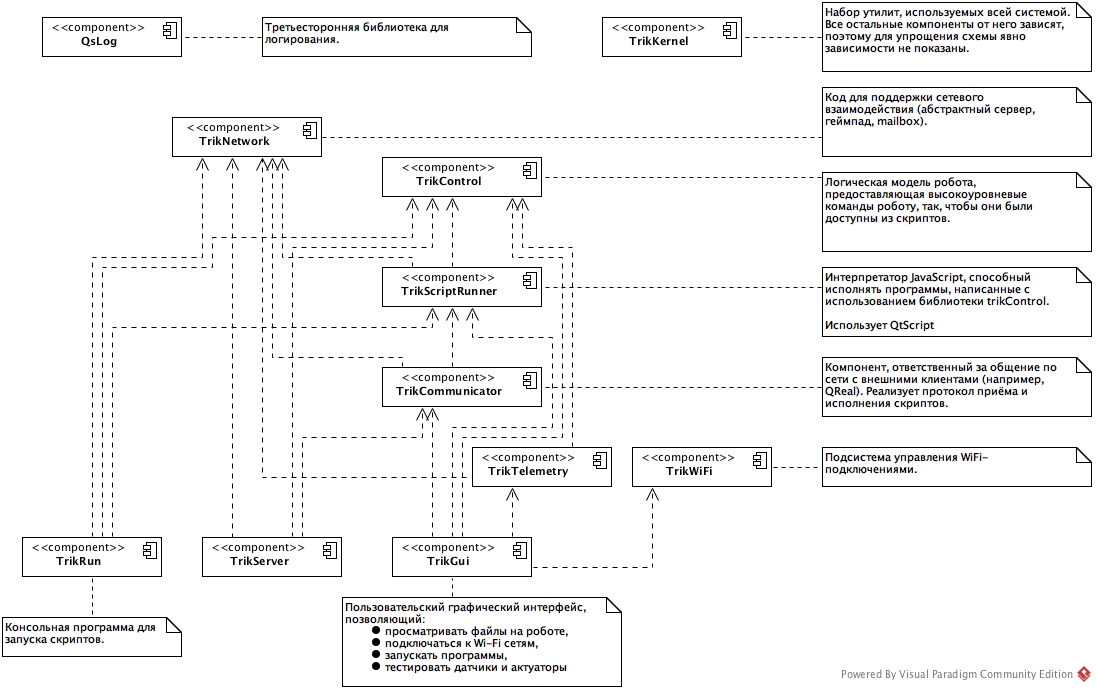
\includegraphics[width=\textwidth]{images/trikRuntime.jpg}
	\caption{Архитектура trikRuntime}
	\label{trikRuntime}
\end{figure}

Основой набора библиотек trikRuntime является библиотека trikControl, предоставляющая API для взаимодействия с сенсорами, актуаторами и другими периферийными частями робота. Ниже перечислены некоторые классы trikControl: Brick — класс, отвечающий за контроллер, инициализирующий периферию робота и дающий к ней доступ, Sensor, ServoMotor и PowerMotor — классы, отвечающие за работу с сенсорами, сервомоторами и силовыми моторами, соответственно. Каждый из них даёт возможность прочитать или выставить значение, что выполняется путём записи или чтения значения в файле, отвечающем за соответствующее устройство.
% * <Роман Белков> 22:37:59 17 May 2017 UTC+0300:
% TODO refactor

% Идеал -- QtScript\footnote{doc.qt.io/qt-4.8/qtscript-module.html}, переименованный в QJSEngine\footnote{doc.qt.io/qt-5/qjsengine.html} с версии Qt 5.0 и уже используемый в основном фреймворке для контроллера TRIK.

% * <Роман Белков> 22:40:12 17 May 2017 UTC+0300:
% trikRuntime программируется с помощью JS
Подробно рассмотрим, как исполняется код на языке JavaScript с помощью компонентов trikRun и trikScriptRunner. Архитектура компонента trikScriptRunner находится на рисунке \ref{trikScriptRunner} (страница \pageref{trikScriptRunner}). trikScriptRunner использует технологию QtScript\footnote{doc.qt.io/qt-4.8/qtscript-module.html} (с версии Qt 5.0 -- QJSEngine\footnote{doc.qt.io/qt-5/qjsengine.html}). QtScript -- это язык программирования, который реализует стандарт ECMAScript\footnote{https://ru.wikipedia.org/wiki/ECMAScript} с расширением в виде поддержки Qt. QtScript практически не отличается от JavaScript с точки зрения пользователя и в то же время позволяет без труда переиспользовать существующий C\texttt{++} код, написанный с использованием Qt. Далее для простоты изложения и в силу вышеописанных изменений с версии Qt 5.0 в тексте не будем отличать QtScript от JavaScript и подразумевать, что JavaScript в контексте данной работы -- это QtScript или JavaScript, использующий QJSEngine.
% * <Роман Белков> 22:43:43 17 May 2017 UTC+0300:
% TODO какие изменения

\begin{figure}[h]
	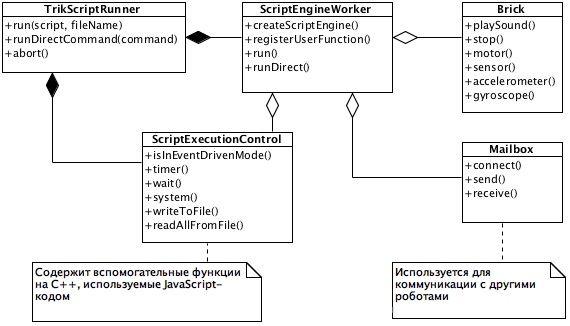
\includegraphics[width=\textwidth]{images/trikScriptRunner.jpg}
	\caption{Архитектура компонента trikScriptRunner}
	\label{trikScriptRunner}
\end{figure}

\subsubsection{TRIK Studio}
TRIK Studio -- это среда визуального и текстового программирования, поддерживающая наиболее популярные в России и Европе образовательные робототехнические платформы: Lego NXT, Lego EV3, TRIK, некоторые версии STM32. В активной стадии разработки -- поддержка большего количества платформ. Поддержка аппаратных платформ осуществляется специальными плагинами. 

Плагин представляет собой генератор или интерпретатор текстового языка программирования. Модульная архитектура плагинов TRIK Studio позволяет легко переиспользовать готовые компоненты, расширяя функциональность при необходимости. Среда предоставляет каркас, необходимый для генераторов: преобразование графа потока управления к представлению, пригодному для генерации структурного кода, подсветку синтаксиса на базе библиотеки QScintilla\footnote{www.riverbankcomputing.com/software/qscintilla/intro}. Фактически, для генераторов необходимо реализовать вручную только текстовые представления конструкций языка программирования и поддержку компилятора (для компилируемых языков). Разнообразие уже созданных генераторов и интерпретаторов языков позволяет без труда понять, как именно создать новый плагин для целевого языка.

Помимо плагинов, поддерживающих генерацию или интерпретацию языков программирования, TRIK Studio обладает инструментами автоматизации и отладки: например, пользователь может из среды загрузить и запустить программу на роботе, а после запуска программы получать вывод программы в консоль TRIK Studio.

\subsubsection{TRIK Stepik checker}
Для популярной платформы онлайн-образования Stepik\footnote{stepik.org} существует вводный курс в робототехнику "Первый шаг в робототехнику" \footnote{stepik.org/462} от методистов TRIK. Для этого курса потребовалось создать специализированную систему, способную проверять решения пользователей на корректность. Так появился TRIK Stepik checker, являющийся выделенной в самодостаточную систему частью TRIK Studio. TRIK Stepik checker способен проверить визуальную диаграмму или код на языке JavaScript.

\subsection{Фреймворки взаимодействия Python и C\texttt{++}}

Существует большое количество наборов библиотек, позволяющих решить задачу использования существующего кода на C\texttt{++} из языка Python. Поскольку ПО контроллера TRIK и среда TRIK Studio являются свободно распространяемым программным обеспечением, в данной работе рассматривались только следующие фреймворки: PyQt, PySide, PythonQt, Boost.Python, SWIG, которые также являются свободно распространяемым ПО.

Прежде, чем приступить к рассмотрению фреймворков взаимодействия, были выделены следующие требования, которым должен удовлетворять выбранный фреймворк.

\begin{itemize}
% * <Роман Белков> 23:11:26 17 May 2017 UTC+0300:
% TODO revise
    \item Возможность поддержать исполнение Python из C\texttt{++} приложения.
    \item Поддержка Qt.
    \item Активная поддержка фреймворка компанией или сообществом.
    \item Доступная документация.
    \item Лицензия с достаточно свободными условиями.
\end{itemize}

\subsubsection{PyQt}

PyQt \cite{pyqt} -- это набор обёрток для фреймворка Qt, который позволяет использовать большую часть функциональности Qt в Python, тем самым достигая TODO

PyQt очень популярен для переиспользования существующих библиотек, написанных на C\texttt{++} с использованием Qt из Python. PyQt не предоставляет возможности для встраивания частей на языке Python в Qt-приложение. Для удобного переиспользования кода на C\texttt{++} существует инструмент SIP\footnote{www.riverbankcomputing.com/software/sip/intro}, который по специальным sip-файлам порождает код обёрток на языке C\texttt{++}. Однако sip-файлы весьма неудобны тем, что являются почти точными копиями заголовочных файлов. Это приводит к тому, что разработчикам приходится изменять sip-файлы при каждом изменении C\texttt{++} кода библиотеки. Более того, SIP обладает весьма слабым парсером языка C\texttt{++}, что не позволяет поддерживать некоторые конструкции динамически. Таким образом, приходиться прибегать к инъекциям в уже сгенерированный код, что является плохой практикой в силу высококих затрат такого подхода на поддержку и высокой вероятности допустить ошибку.

\subsubsection{PySide}
PySide -- это набор обёрток для фреймворка Qt. Проект PySide стартовал как аналог PyQt и практически не отличается от PyQt. Единственное значимое отличие -- PyQt распространяется под коммерческой или GPLv3 лицензией, в то время как PySide распространяется под LGPL лицензией, что позволяет использовать его с большей свободой. 

Плюсом фреймворка является то, что Qt Company\footnote{en.wikipedia.org/wiki/The\_Qt\_Company} официально поддерживает PySide, что обеспечивает активную разработку набора библиотек. 

Однако, данный продукт не обладает актуальной документацией, что затрудняет его использование. Также стоит отметить, что PySide на данный момент поддерживает меньшую часть набора библиотек Qt по сравнению с PyQt.

\subsubsection{PythonQt}
PythonQt -- это библиотека для Qt, нацеленная на встраивание Python в С++/Qt приложение. PythonQt разрабатывался для платформы MeVisLab\footnote{www.mevislab.de} с целью предоставления возможности использования Python-кода для расширения возможностей платформы или специальной обработки информации \cite{heckelMeVisLab}. 

Для использования PythonQt необходимо в C\texttt{++} коде описать обёртку необходимого объекта и зарегистрировать её в желаемом модуле Python. Для упрощения данной работы PythonQt имеет генератор, способный по заголовочным файлам C\texttt{++} и системе типов сгенерировать все необходимые обёртки. Хотя генератор находится в разработке и не содержит некоторых необходимых функций, анализ кода генератора показал, что временные затраты на доработку его до состояния, необходимого для данной работы, приемлемы.

\subsubsection{Boost.Python}
Boost.Python \cite{abrahams2003boost} -- это библиотека для взаимодействия C\texttt{++} и Python, позволяющая использовать скрипты на языке Python как часть программы, написанной на C\texttt{++}. 

Основная цель Boost.Python -- предоставить возможность переиспользовать код, написанный на C\texttt{++}, в коде, написанном на Python, средствами лишь компилятора C\texttt{++}. Это отличает его от, например, SIP, который использует специальный язык для создания промежуточной коммуникации. При этом в Boost.Python учитываются основные различия между двумя языками и предоставлены интерфейсы для удобного взаимодействия.

Boost.Python предлагает возможность интерпретации Python 
% * <Роман Белков> 23:28:58 17 May 2017 UTC+0300:
% TODO

Для автоматизации процесса создания обёрток над кодом существуют следующие инструменты: Pyste и Py++. Pyste\footnote{www.boost.org/doc/libs/1\_60\_0/libs/python/pyste/doc/running\_pyste.html} -- генератор обёрток для Boost.Python, который был разработан, как часть фреймворка Boost.Python. Разработка была прекращена в 2011 году. Pу++\footnote{bitbucket.org/ompl/pyplusplus} -- генератор обёрток для Boost.Python, используемый в популярной библиотеке планирования движения OMPL\cite{sucan2012theOMPL}. В отличие от Pyste, Py++ поддерживается разработчиками OMPL и, следовательно, может быть использован при разработке новых проектов с использованием Boost.Python.
% Более того, Pyste использует GCC-XML\cite{gccxml}, разработка которого официально остановилась в 2015 году\footnote{gccxml.github.io/HTML/News.html}. 


Однако, поскольку Boost.Python разрабатывался для работы с чистым С++ кодом, то в нём отсутствует поддержка фреймворка Qt. Это не позволяет использовать сигналы и слоты Qt из Python, что является недостатком. 

% The primary goal of Boost.Python is to allow users to expose C\texttt{++} classes and functions to Python using nothing more than a C\texttt{++} compiler. In broad strokes, the user experience should be one of directly manipulating C\texttt{++} objects from Python.

% However, it's also important not to translate all interfaces too literally: the idioms of each language must be respected. For example, though C\texttt{++} and Python both have an iterator concept, they are expressed very differently. Boost.Python has to be able to bridge the interface gap.

% It must be possible to insulate Python users from crashes resulting from trivial misuses of C\texttt{++} interfaces, such as accessing already-deleted objects. By the same token the library should insulate C\texttt{++} users from low-level Python 'C' API, replacing error-prone 'C' interfaces like manual reference-count management and raw PyObject pointers with more-robust alternatives.

% Support for component-based development is crucial, so that C\texttt{++} types exposed in one extension module can be passed to functions exposed in another without loss of crucial information like C\texttt{++} inheritance relationships.

% Finally, all wrapping must be non-intrusive, without modifying or even seeing the original C\texttt{++} source code. Existing C\texttt{++} libraries have to be wrappable by third parties who only have access to header files and binaries.

\subsubsection{SWIG}
TODO выкинуть SWIG

\subsection{Выбор фреймворка}

Таблица \ref{table:frameworkComparison} (страница \pageref{table:frameworkComparison})

Сначала PyQt, потом PythonQt

% \begin{table}[]
% \centering
% \resizebox{\textwidth}{!}{%
% \begin{tabular}{|l|c|c|c|c|c|}
% \hline
%                                                                               & PyQt & PySide & PythonQt & SWIG & Boost.Python \\ \hline
% поддержка Qt                                                                  & +    & +      & +        & +/-  & -            \\ \hline
% \begin{tabular}[c]{@{}l@{}}поддержка фреймворка\\ разработчиками\end{tabular} & +    & -      & -        & +    & +            \\ \hline
% доступная документация                                                        & +    & -      & -        & +    & +            \\ \hline
% \end{tabular}%
% }
% \caption{Сравнение фреймворков}
% \label{table:frameworkComparison}
% \end{table}

\begin{table}[]
\centering
\resizebox{\textwidth}{!}{%
\begin{tabular}{|l|c|c|c|c|c|}
\hline
                                                                          & PyQt                                                          & PySide & PythonQt & SWIG & Boost.Python  \\ \hline
встраивание Python в C\texttt{++}                                                  & -                                                             & -      & +        & -    & +             \\ \hline
поддержка Qt                                                              & +                                                             & +      & +        & -    & -             \\ \hline
\begin{tabular}[c]{@{}l@{}}поддержка фреймворка\end{tabular} & +                                                             & -      & -        & +    & +             \\ \hline
хорошая документация                                                      & +                                                             & -      & -        & +    & +             \\ \hline
обёртка C\texttt{++} для Python                                                    & +                                                             & +      & -        & +    & +             \\ \hline
лицензия                                                                  & \begin{tabular}[c]{@{}c@{}}GPL + \\ коммерческая\end{tabular} & LGPL   & LGPL     & GPL  & Boost.License \\ \hline
\end{tabular}%
}
\caption{Сравнение фреймворков}
\label{table:frameworkComparison}
\end{table}

\section{Разработка требований}
Прежде, чем приступить к проектированию программного обеспечения, необходимо выявить требования заказчиков и будущих пользователей нового образовательного решения, а также оценить объёмы работ и риски, связанные с разработкой программного обеспечения, позволяющего использовать Python в образовательных решениях TRIK. 

Cценарии использования основного образовательного решения TRIK представлены на рисунке \ref{usecases} (страница \pageref{usecases}).

\begin{figure}[h]
	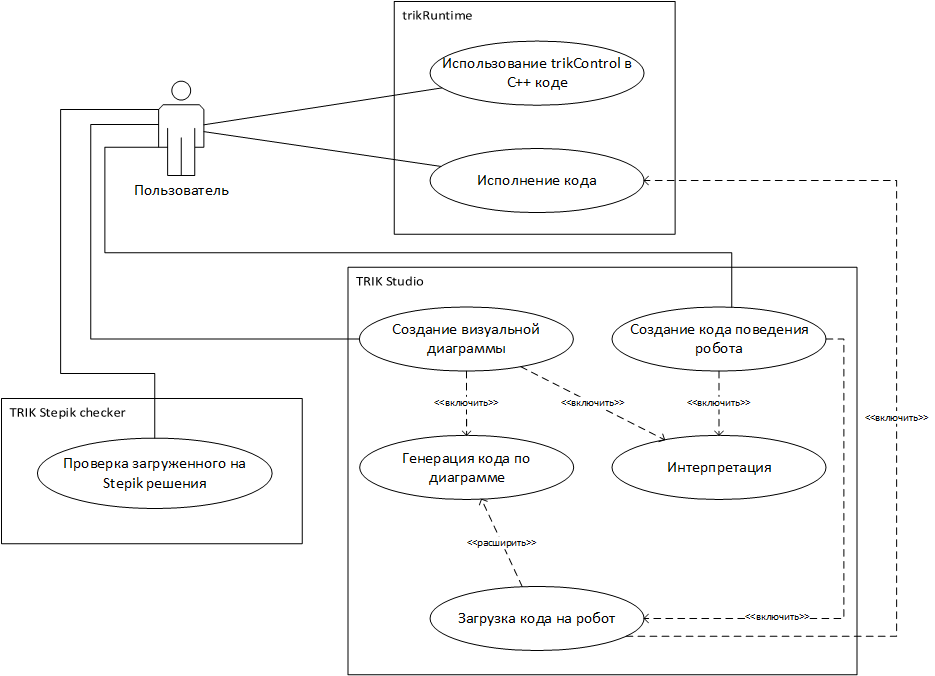
\includegraphics[width=\textwidth]{images/diploma-usecase.png}
	\caption{Сценарии использования образовательного решения TRIK}
	\label{usecases}
\end{figure}

Таким образом, были выделены следущие согласованные требования:
\begin{itemize}
    \item В сжатые сроки (один месяц) предоставить версию продукта, обладающую минимальной необходимой функциональностью.
    \item Учитывать затраты на сопровождение решения.
    \item Обеспечить одинаковое поведение при использовании Python в 2D модели или на реальном роботе.
\end{itemize}

\section{Архитектура}

Поскольку одним из требований к техническому решению была разработка версии продукта, обладающего минимальной функциональностью, было принято решение разрабатывать техническое решение в два этапа:
\begin{enumerate}
    \item Разработка технического решения с минимальной функциональностью
    \begin{itemize}
        \item Создание обёртки trikRuntime для использования с PyQt
        \item Реализация генератора Python в TRIK Studio
    \end{itemize}
    \item Разработка функциональности, аналогичной QtScript в trikScriptRunner
    \begin{itemize}
        \item Использование PythonQt для встраивания в trikRuntime
        \item Реализация интерпретации Python 2D моделью робота
    \end{itemize}
\end{enumerate} 

Такой подход был выбран потому, что хотя PythonQt или Boost.Python и являются наиболее подходящими фреймворками для решения данной задачи, оба фреймворка обладают недостатками, для устранения которых потребовалось бы значительное количество времени. 
% * <Роман Белков> 23:41:58 17 May 2017 UTC+0300:
% TODO

Это позволило добиться более естественной интеграции наподобие той, что предлагает QtScript. Более того, пользователям TRIK, привыкшим работать с JavaScript, не придётся привыкать к системе с новым usage flow TODO. 

\subsection{Робот TRIK}
Разработка программного обеспечения для робота представляла наибольшую трудность. Именно из-за сложности реализации данной компоненты было принято решение разработки системы в два этапа. По результатам обзора PythonQt или Boost.Python являлись наиболее подходящими фреймворками для решения данной задачи, но оба фреймворка обладали недостатками, для устранения которых потребовалось бы значительное количество времени: Boost.Python не хватало поддержки Qt и её пришлось реализовать в рамках данной работы, а PythonQt были необходимы патчи к генератору.   

\subsection{TRIK Studio}

\subsection{TRIK Stepik Checker}


% \section{Особенности реализации}

\section{Апробация}
В качестве проверки применения представленного технического решения были проведены несколько экспериментов, тестирующих части системы отдельно и в комплексе. Был успешно проверен переписаннный с JavaScript на Python код некоторых демонстрационных моделей TRIK: светового меча и дистанционно управляемой тележки. Также была проверена работоспособность кодогенератора Python на всех базовых примерах, поставляемых с TRIK Studio. Полученный порождённый код успешно запускался на роботе TRIK. 

Таким образом, в ходе апробации части системы и система в целом были протестированы, а полученный код моделей может быть использован для регрессионного тестирования представленного в данной работе технического решения.

\section{Документация}
Поскольку образовательные решения TRIK ориентированы в том числе и на школьников средних и старших классов, одним из важным моментов при создании описанной системы было написание базовой документации и создание примеров программ для наглядности. Это упростило работу методистов и позволило первым пользователям быстрее разобраться с представленной системой. TODO


% У заключения нет номера главы
\section*{Заключение}

В рамках данной работы были получены следующие результаты.
\begin{enumerate}
\item Сделан обзор архитектуры существующего ПО образовательных решений TRIK.
\item Определены требования к программному решению.
\item Разработана архитектура программного решения.
\item Выполнена реализация программного решения.
\item Разработанное программное решение внедрено в образовательные решения TRIK.
\end{enumerate}


В ходе работы промежуточные результаты представлялись докладом на VII Всероссийской конференции "Современное технологическое обучение: От компьютера к роботу", а также докладом на всероссийской конференции "СПИСОК-2017".

Существует несколько направлений дальнейшего развития полученных результатов. Например, возможно создание полноценного аналога QJSEngine для языка Python.

\setmonofont[Mapping=tex-text]{CMU Typewriter Text}
\bibliographystyle{ugost2008ls}
\bibliography{diploma.bib}
\end{document}